\documentclass{article}

% Packages for math and formatting
\usepackage{amsmath, amssymb}
\usepackage{geometry}
\usepackage{graphicx}
\usepackage{bm}
\usepackage{physics}


% Page setup
\geometry{margin=1in}

\begin{document}

\subsection{Focal Length}
A set of parallel lines is parallel to the ray connecting the optical center and their vanishing point. 
If the vanishing point appears at pixels $(x, y)$ on the image with optical center $(x_c, y_c)$, then 
the ray is characterized by the homogenous coordinates
$$ 
\begin{bmatrix}
    x - x_c \\
    y - y_c \\ 
    f
\end{bmatrix}
$$

(assuming aspect ratio of 1). 
We also know that two rays may be orthogonal in 3D space is the lines parallel to each of them are orthogonal. 
Thus, let $(x_1, y_1), (x_2, y_2)$ be the vanishing points of two orthogonal set of parallel lines, 
we have 
\begin{align*}
    (x_1 - x_c, y_1 - y_c, f) \cdot (x_2 - x_c, y_2 - y_c, f) = 0 \Leftrightarrow\\
    f^2 = -(x_1 - x_c)(x_2 - x_c) - (y_1 - y_c)(y_2 - y_c)
\end{align*}

\subsection{Height}

\begin{figure}[h]
    \centering
    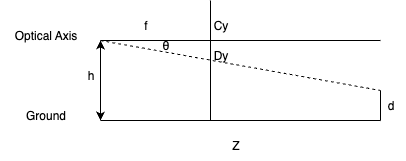
\includegraphics[width=0.7\textwidth]{height-estimation.drawio.png} % omit .svg extension
    \caption{Height Estimation. $f$ the focal length, $Z$ the distance of the object,
    $C_y$ and $D_y$ the $y$ pixel coordinate of the optical axis and ray connecting the object head, respectively.}
    \label{fig:example}
\end{figure}

Without additional information, the real size of objects in the image is only determined up to scale. However, we can camera height given an object of 
known height at a known distance, illustrated from the image above. 
We have 
with 
$$
\theta = tan^{-1}(\frac{D_y - C_y}{f})
$$

$$
h = d - Z \sin \theta
$$

\end{document}